% lint-skip: 未完成ステータス（figure/table caption 未対応，人手チェック時に解消予定）
\documentclass[../../main.tex]{subfiles}
\begin{document}

\begin{flushright}
  \footnotesize\textit{【自動文字起こし・要確認】}
\end{flushright}

{\bf [解答]} $f(x) = x^3 + ax$, $P$の$x$座標を$t$とすると, $f'(t) = 3t^2 + a$から接線$l$は
$$ l: y = g(x) = (3t^2 + a)x - 2t^3 $$
だから
$$ f(x) - g(x) = x^3 - 3t^2x + 2t^3 = (x-t)^2(x+2t) $$
より, $x = -2t$ ($x \neq t$, $\because t \neq 0$) を$x$座標とする点$Q$で交わる \dots (1)

\paragraph{(2)}

$x \le 0$の部分の面積$S_1$, $x \ge 0$ " $S_2$とする．$y = f(x)$は原点対称性だから$t>0$の時 $S_1 : S_2 = A : B$ なら$t<0$の時$S_1 : S_2 = B : A$である \dots (1)
よって, $t>0$の時のみ考える．

$$ S_1 = \int_{-2t}^0 \{ f(x) - g(x) \} dx $$
$$ = \int_{-2t}^0 \{ (x+2t) - 3t \}^2 (x+2t) dx $$
$$ = \left[ \dfrac{1}{4} (x+2t)^4 - 2t(x+2t)^3 + \dfrac{9t^2}{2} (x+2t)^2 \right]_{-2t}^0 $$
$$ = \left( \dfrac{16}{4} - 16 + 18 \right) t^4 = 6t^4 \cdots \text{(2)} $$

$$ S_2 = \int_0^t \{ f(x) - g(x) \} dx = \int_0^t (x-t)^2 (x+2t) dx $$
$$ = \left[ \dfrac{1}{4} (x-t)^4 + t (x-t)^3 \right]_0^t $$
$$ = -\dfrac{1}{4} t^4 + t^4 = \dfrac{3}{4} t^4 \cdots \text{(3)} $$

\begin{figure}[htb]
  \centering
  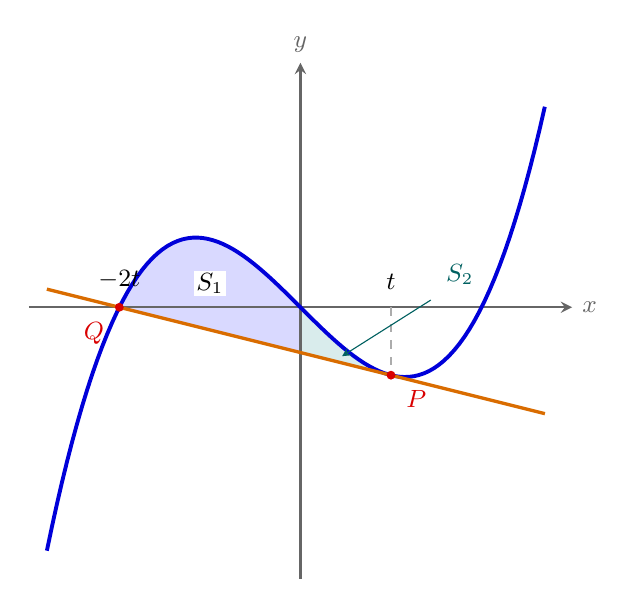
\begin{tikzpicture}[x=2.3cm, y=2.3cm, >=stealth,
    every node/.style={font=\small}]
    % Example: t=1/2, a=-1, f(x)=x^3-x, g(x)=-x/4-1/4.
    \fill[blue!15]
    plot[domain=-1:0, samples=50] (\x,{\x*\x*\x-\x}) --
    plot[domain=0:-1, samples=2] (\x,{-0.25*\x-0.25}) -- cycle;
    \fill[teal!15]
    plot[domain=0:0.5, samples=30] (\x,{\x*\x*\x-\x}) --
    plot[domain=0.5:0, samples=2] (\x,{-0.25*\x-0.25}) -- cycle;
    \draw[->, thick, gray!80!black] (-1.5,0) -- (1.5,0)
    node[right] {$x$};
    \draw[->, thick, gray!80!black] (0,-1.5) -- (0,1.35)
    node[above] {$y$};
    \draw[line width=1.4pt, blue!85!black,
    domain=-1.4:1.35, samples=100]
    plot (\x,{\x*\x*\x-\x});
    \draw[line width=1.2pt, orange!85!black,
    domain=-1.4:1.35, samples=2]
    plot (\x,{-0.25*\x-0.25});
    \draw[dashed, gray!65] (0.5,0) -- (0.5,-0.375);
    \fill[red!85!black] (-1,0) circle (1.6pt);
    \fill[red!85!black] (0.5,-0.375) circle (1.6pt);
    \node[below left=2pt, red!85!black] at (-1,0) {$Q$};
    \node[below right=2pt, red!85!black] at (0.5,-0.375) {$P$};
    \node[above=3pt] at (0.5,0) {$t$};
    \node[above=3pt] at (-1,0) {$-2t$};
    \node[fill=white, inner sep=1pt] at (-0.5,0.13) {$S_1$};
    \draw[->, thin, teal!75!black] (0.72,0.04) -- (0.23,-0.27);
    \node[above right=2pt, teal!75!black] at (0.72,0.04) {$S_2$};
  \end{tikzpicture}
  \caption{曲線 $y=f(x)$ と接線の間の面積 $S_1,S_2$（$t=1/2$ の例）}
\end{figure}

(2), (3), $t \neq 0$ から, $t>0$の時, $S_1 : S_2 = 8 : 1$
$t<0$ " $S_1 : S_2 = 1 : 8 \quad (\because \text{(1)})$

\end{document}
